\documentclass{beamer}
\usepackage[utf8]{inputenc}
\usepackage[T1]{fontenc}
\usepackage[english]{babel}
\usepackage{graphicx}
\usepackage{times}

\usetheme{AGH}

\title[]{
	Managing data availability and integrity\\
	in federated cloud storage}
\subtitle[]{
	Zarządzanie dostępnością i integralnością danych\\
	w sfederowanych zasobach chmury obliczeniowej.
}

\author[Krzysztof Styrc]{Krzysztof Styrc}

\date[]{11.12.2011}

\institute[Informatyka AGH]
{
\\
\noindent
Promotor: dr inż. Marian Bubak (AGH)\\
\noindent
Konsultant: Piotr Nowakowski (ACC Cyfronet)
}

\setbeamertemplate{itemize item}{$\maltese$}

\begin{document}

{
%\usebackgroundtemplate{\includegraphics[width=\paperwidth]{titlepage}} % wersja angielska
\usebackgroundtemplate{\includegraphics[width=\paperwidth]{titlepagepl}} % wersja polska
 \begin{frame}
   \titlepage
 \end{frame}
}

%---------------------------------------------------------------------------


\begin{frame}
\frametitle{Krótko o projekcie VPH-Share}

\begin{block}{Projekt VPH-Share ma na celu:}
\begin{itemize}
	\item stworzenie platformy typu cloud dla potrzeb sektora medycznego
	\item umożliwiającej udostępnianie i wymianę danych oraz wiedzy,
	\item której jednym z wymagań jest ich wiarygodność i integralność.
\end{itemize}
\end{block}

\begin{block}{Komponent Data Reliability and Integrity(DRI) ma za zadanie:}
\begin{itemize}
	\item okresowe sprawdzanie wiarygodności i integralności danych,
	\item umożliwiać replikację danych na różne platformy cloudowe,
	\item śledzić historię i pochodzenie plików z danymi.
\end{itemize}
\end{block}

\end{frame}

%---------------------------------------------------------------------------

\begin{frame}
\frametitle{Wiarygodność i integralność pliku}

\begin{block}{Temat dobrze zbadany:}
\begin{itemize}
	\item funkcje skrótu(MD5, SHA-1),
	\item Message Authentication Code(MAC),
	\item Error Correcting Code(ECC).
\end{itemize}
\end{block}

\begin{block}{Nowe wyzwania - cloud storage:}
\begin{itemize}
	\item przechowywanie bardzo dużych zbiorów danych,
	\item przechowywanie danych na obcych zasobach,
	\item brak gwarancji wiarygodności i integralności.
\end{itemize}
\end{block}

\end{frame}

%---------------------------------------------------------------------------

\begin{frame}
\frametitle{Wiarygodność i integralność pliku}

\begin{block}{Konsekwencje przechowywania danych w chmurze:}
\begin{itemize}
	\item brak gwarancji wiarygodności i integralności,
	\item nieefektywność zewnętrznej walidacji - duże zbiory danych,
\end{itemize}
\end{block}

\begin{block}{Proof of Retrievability(POR):}
\begin{itemize}
	\item walidacja tylko po części zawartości pliku,
	\item plik jest przechowywany w formie zmodyfikowanej,
	\item poprawność oparta o zastosowanie funkcji skrótu, MAC i ECC,
	\item sumy kontrolne w większości wbudowane w plik(modyfikacja).
\end{itemize}
\end{block}

\end{frame}

%---------------------------------------------------------------------------

\begin{frame}
\frametitle{Ogólny schemat systemu POR}

\begin{figure}
\includegraphics[width=0.9\textheight]{por.png}
\end{figure}

\end{frame}

%---------------------------------------------------------------------------

\begin{frame}
\frametitle{Modyfikacja ECC + MAC}

\begin{block}{Zmodyfikowany plik $F^{*}$ może wyglądać następująco:}
\begin{figure}
\includegraphics[width=\textwidth]{modified_file.png}
\end{figure}
\end{block}

\end{frame}

%---------------------------------------------------------------------------

\begin{frame}
\frametitle{Wiarygodność i integralność w VPH-Share}

\begin{block}{Wymagania platformy VPH-Share:}
\begin{itemize}
	\item przechowywanie plików w postaci niezmodyfikowanej,
	\item sumy kontrolne przechowywane w rejestrze Atmosphere, a nie zawarte w pliku - rejestr ma ograniczone rozmiary!
\end{itemize}
\end{block}

\begin{block}{Cel pracy:}
\begin{itemize}
	\item opracowanie algorytmu walidacji w oparciu o podejście POR, który uwzględniałby powyższe wymagania i ograniczenia,
	\item porównanie różnych algorytmów i wybranie tego, który da najlepszą wykrywalność błędów,
	\item implementacja komponentu walidacji DRI w oparciu o ten algorytm.
\end{itemize}
\end{block}

\end{frame}

%---------------------------------------------------------------------------

\begin{frame}
\frametitle{Bibliografia}

\begin{itemize}
	\item VPH-Share Deliverable 2.1
	\item VPH-Share Deliverable 2.2
	\item PORs: Proofs of Retrievability for Lare Files - Juels, Kaliski,
	\item HAIL: A High Availability and Integrity Layer for Cloud Storage - Juels, Bowers, Oprea
	\item Venus: Verification for Untrusted Cloud Storage - wielu autrów
\end{itemize}

\end{frame}

\begin{frame}
\frametitle{Aktualna architektura}

\begin{figure}
\includegraphics[width=0.8\textwidth]{schemat.pdf}
\end{figure}
\end{frame}

\begin{frame}
\frametitle{Opis serwisów i integracji}

\begin{block}{Opis serwisów:}
\begin{itemize}
	\item DRI Service -- serwis do walidacji danych,
	\item Swift BlobStore -- przechowuje dane z zapewnieniem replikacji,
	\item Metadata Registry -- baza metadanych obiektów z BlobStore,
\end{itemize}
\end{block}

\begin{block}{Integracja:}
\begin{itemize}
	\item Swift BlobStore -- udostępnia interfejs REST API, istnieje świetna biblioteka JClouds dostępu do Cloud Storage,
	\item Metadata Registry -- wewnętrzna implementacja projektu VPH-Share, udostępnia interfejs REST API, integracja możliwa za pomocą JAX-RS.
\end{itemize}
\end{block}
\end{frame}

\begin{frame}
\frametitle{Algorytm walidacji}

\begin{block}{Algorytm walidacji:}
\begin{enumerate}
	\item pobierz metadane zbioru danych(nazwa kontenera, nazwy plików, wartości skrótów, itp) z Metadata Registry,
	\item dla każdego pliku ze zbioru pobierz potrzebne dane do obliczenia wartości skrótu ze Swift BlobStore,
	\item dla każdego pliku porównaj otrzymaną wartość skrótu z wartością zapisaną w metadanych.
\end{enumerate}
\end{block}
\end{frame}

\begin{frame}
\frametitle{Ocena wydajności systemu}

\begin{block}{Przykładowy zbiór:}
\begin{itemize}
	\item zbiór zawiera $64K$ plików,
	\item średnia wielkość pliku $\sim 0.5MB$,
	\item wielkość zbioru $\sim 32GB$,
\end{itemize}
\end{block}

\begin{block}{Obliczenia:}
\begin{itemize}
	\item obliczanie skrótow MD5/SHA1 ma większą przepustowość niż transfer sieciowy,
	\item największy narzut -- transfer sieciowy,
	\item załóżmy transfer $5MB/s$,
	\item czas przesyłu $\sim 1.8h$!
\end{itemize}
\end{block}
\end{frame}

\begin{frame}
\frametitle{Problemy, problemy}
\begin{block}{Problemy, problemy:}
\begin{itemize}
	\item pożądane byłoby pobranie wszystkich potrzebnych do walidacji fragmentów w jednym żądaniu HTTP,

	\textit{np. zwróć mi bajty 5-10, 45-50, 95-100, itd.}
	\item rozwiązanie: użycie nagłówka HTTP Range w celu określenia żądanych fragmentów pliku,

	\textit{np. Range:5-10,45-50,95-100,...}	
	\item niestety: Openstack Swift aktualnie nie wspiera w pełni nagłówka Range, możliwe jest określenie wyłącznie pojedyńczego fragmentu,

	\textit{np. Range:5-10}
\end{itemize}
\end{block}
\end{frame}

\begin{frame}
\frametitle{Problemy, Problemy}
\begin{block}{Pomysły na rozwiązanie}
\begin{itemize}
	\item zwrócić się do twórców Openstack Swift o implementację pełnego wsparcia nagłówka HTTP Range -- niestety przy obsłudze HTTP Openstack korzysta z biblioteki \textit{Webob}, a znowu jej twórcy stwierdzili, że nie znają sensownego zastosowania pełnego nagłówka HTTP Range poza opublikowanym atakiem DDoS na Apache Server,
	\item wysyłanie osobnych żądań HTTP o każdy fragment -- nieskalowalne, zalewa serwer żądaniami, w znacznym stopniu ograniczyłoby to liczbę fragmentów na podstawie których obliczany jest skrót pliku,
	\item ściąganie całości pliku -- jak wykazała moja krótka analiza wydajnościowa, nieakceptowalne.
\end{itemize}
\end{block}
\end{frame}

\begin{frame}
	\titlepage
\end{frame}

\begin{frame}
\frametitle{Architektura DRI}
\begin{figure}
\includegraphics[width=0.8\textwidth]{schemat.pdf}
\end{figure}
\end{frame}

\begin{frame}
\frametitle{Wymagania projektu}
\begin{block}{Wymagania funkcjonalne:}
\begin{itemize}
	\item periodyczne sprawdzanie dostępności i integralności danych (walidacja),
	\item przeprowadzenie walidacji na żądanie użytkownika,
	\item replikacja danych w federacji cloudów,
	\item śledzenie historii i pochodzenia danych binarnych.
\end{itemize}
\end{block}
\end{frame}
\begin{frame}
\frametitle{Wymagania projektu}
\begin{block}{Wymagania niefunkcjonalne:}
\begin{itemize}
	\item efektywność walidacji danych,
	\item bezpieczeństwo serwisu DRI,
	\item skalowalność rozwiązania,
	\item możliwość konfiguracji parametrów.
\end{itemize}
\end{block}
\end{frame}

\begin{frame}
\frametitle{Przypadki użycia}
\begin{block}{Użytkownik dodaje zbiór do walidacji}
\begin{enumerate}
	\item pobranie metadanych zbioru danych z rejestru AIR,
	\item obliczenie sum kontrolnych,
	\item aktualizacja zbioru danych w rejestrze AIR,
	\item dodanie zbioru do periodycznej walidacji,
\end{enumerate}
w przypadku błędu zwrócenie go użytkownikowi.
\end{block}
\end{frame}

\begin{frame}
\frametitle{Przypadki użycia}
\begin{block}{Użytkownik dokonuje walidacji zbioru danych:}
\begin{enumerate}
	\item pobranie metadanych zbioru danych z rejestru AIR,
	\item sprawdzenie dostępności i integralności zbioru danych,
	\item wysłanie informacji o statusie walidacji do serwisu notyfikacji.
\end{enumerate}
\end{block}
\end{frame}

\begin{frame}
\frametitle{Przypadki użycia}
\begin{block}{Użytkownik dokonuje replikacji zbioru danych:}
\begin{enumerate}
	\item pobranie metadanych zbioru danych z rejestru AIR,
	\item sprawdzenie ograniczeń zbioru danych, 
	\item replikacja zbioru danych na wybrany cloud,
	\item wysłanie informacji o zakończeniu do serwisu notyfikacji,
\end{enumerate}
w przypadku błędu wysłanie błędu do serwisu notyfikacji.
\end{block}
\end{frame}

\begin{frame}
\frametitle{Interfejs serwisu DRI}
\begin{figure}
\includegraphics[width=1.0\textwidth]{dri_interface.png}
\end{figure}
\end{frame}

\begin{frame}
\begin{figure}
\includegraphics[width=0.85\textheight]{dri-service.png}
\end{figure}
\end{frame}

\begin{frame}
\frametitle{}
\begin{block}{Używane technologie:}
\begin{itemize}
	\item Java - język implementacji,
	\item JAX-RS i Jersey - interfejs REST serwisu,
	\item Jclouds - jednolity dostęp do różnych platform cloudowych,
	\item Google Guava i Guice, Apache Commons,
	\item Apache Tomcat, Maven, SVN.
\end{itemize}
\end{block}
\end{frame}

\begin{frame}
\frametitle{Użytkownik dodaje zbiór do walidacji}
\begin{figure}
\includegraphics[width=0.8\textwidth]{registration-diagram.png}
\end{figure}
\end{frame}

\begin{frame}
\frametitle{Użytkownik dokonuje walidacji zbioru danych}
\begin{figure}
\includegraphics[width=1.0\textwidth]{validation-diagram.png}
\end{figure}
\end{frame}

\begin{frame}
\frametitle{Użytkownik dokonuje replikacji zbioru danych}
\begin{figure}
\includegraphics[width=0.8\textwidth]{replication-diagram.png}
\end{figure}
\end{frame}

\begin{frame}
\begin{block}{Stan prac:}
\begin{itemize}
	\item periodyczna walidacji zbiorów danych,
	\item walidacja danych na żądanie,
	\item walidacja oparta o SHA-1,
	\item notyfikowanie o statusie walidacji,
	\item gotowa integracja z resztą projektu VPH-Share,
	\item \textbf{czas na implementację efektywnych algorytmów walidacji.}
\end{itemize}
\end{block}
\end{frame}


%---------------------------------------------------------------------------

\section*{Bibliography}
\nocite{*}
%\bibliographystyle{plplain}
\bibliography{biblio}

\end{document}

